\chapter{Descrição do Projeto}\label{descricao}

\section{Materiais Utilizados}

\begin{table}[H]
\centering
\caption{Materiais utilizados no projeto.}
\label{tab:materiais}
\begin{tabular}{lrr}
\multicolumn{1}{l}{\textbf{Materiais}} & \multicolumn{1}{l}{\textbf{Quantidade}} & \multicolumn{1}{l}{\textbf{Custos (R\$)}} \\\toprule
Algodão                   & 3 pacotes   & 4,00 pacote  \\
Arruelas                  & 12 unidades & 0,50 unidade \\
Barras de metal           & 2 unidades  & -            \\
Garrafa PET               & 1 unidade   & -            \\
Graxa                     & 6 latas     & 7,00 lata    \\
Mangueira                 & 1 metro     & 4,00 metro   \\
Parafuso de rosca sem fim & 2 metros    & 2,00 metro   \\
Placas de madeira         & 2 unidades  & -            \\
Porcas                    & 12 unidades & 0,50 unidade \\
Silicone                  & 1 frasco    & 14,00 frasco \\ \bottomrule
\end{tabular}
\end{table}

\section{Montagem}
\label{sec:montagem}

Primeiramente, foram realizados quatro furos nos cantos das placas de madeira,
onde os parafusos seriam acoplados para unir o sistema. Em uma das placas de
madeira, foi feito um furo central de \nicefrac{1}{4} \si{in}, para encaixe da
mangueira de alimentação do filtro. Na montagem da membrana filtrante (latas
preenchidas com algodão), foram feitos furos de \nicefrac{1}{4} \si{in} no
centro de cada lata, por onde a solução a ser filtrada entraria no meio
filtrante (algodão).

Foram conectadas as duas placas por meio dos parafusos de rosca sem fim, de modo
a deixar um espaço para colocar as membranas filtrantes. As latas foram
preenchidas com algodão e tampadas, em seguida, foram empilhadas e acopladas
entre as duas placas de madeira, de modo que as membranas filtrantes ficaram
prensadas entre as placas de madeira. Uma mangueira foi conectada ao furo
central da placa de madeira, por onde seria feita a alimentação. Foi utilizada
uma garrafa PET para colocar a solução a ser filtrada.

\begin{figure}
  \begin{subfigure}[H]{0.4\textwidth}
    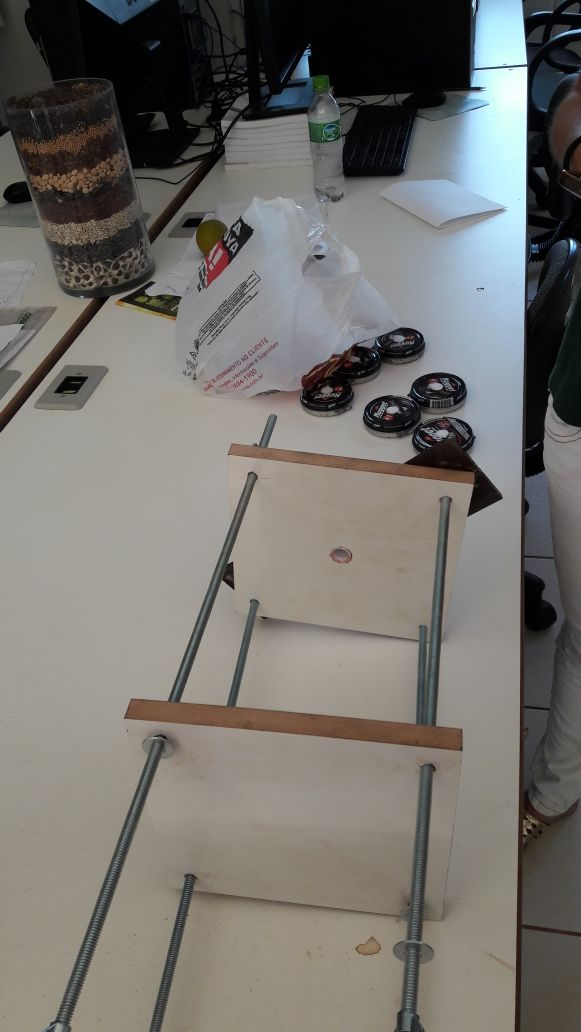
\includegraphics[width=\textwidth]{figuras/montagem1.png}
    \caption{Estrutura de madeira com os parafusos.}
  \end{subfigure}%
  \hfill
  \begin{subfigure}[H]{0.4\textwidth}
    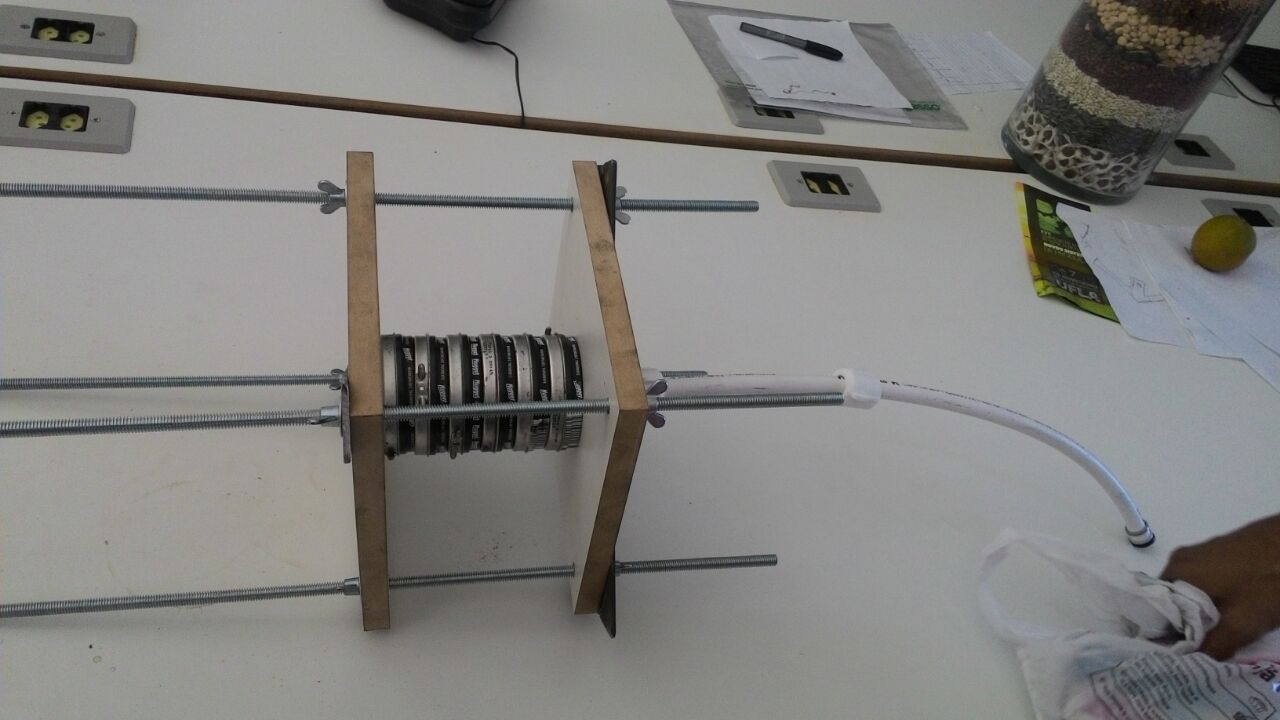
\includegraphics[width=\textwidth]{figuras/montagem2.png}
    \caption{Estrutura prensando as latas. A magueira branca é a alimentação.}
  \end{subfigure}%
  \caption{Montagem}
\end{figure}


%%% Local Variables:
%%% mode: latex
%%% TeX-master: "../main_archive"
%%% End:
